\documentclass[12pt]{article}
\usepackage[spanish]{babel}
\usepackage{natbib}
\usepackage{url}
\usepackage[utf8x]{inputenc}
\usepackage{amsmath}
\usepackage{float}
\usepackage{subfig}
\usepackage{graphicx}
\graphicspath{{images/}}
\usepackage{parskip}
\usepackage{fancyhdr}
\usepackage{vmargin}
\usepackage{mathtools}
\usepackage{amssymb} 



\title{Actividad \#2: Elementos de programaciòn Python }							
\author{\Large Jesùs Valenzuela Nieblas\\}											
\date{\today} 

\makeatletter
\let\thetitle\@title
\let\theauthor\@author
\let\thedate\@date										
\makeatother

\pagestyle{fancy}

\lhead{\thetitle}
\rhead{}
\cfoot{\thepage}

\begin{document}

%%%%%%%%%%%%%%%%%%%%%%%%%%%%%%%%%%%%%%%%%%%%%%%%%%%%%%%%%%%%%%%%%%%%%%%%%%%%%%%%%%%%%%%%%

\begin{titlepage}
	\centering
    \vspace*{.5cm}
     
\includegraphics[scale = 0.7]{logo}\\	% University Logo
    \textsc{\Large Universidad de Sonora}\\[1.0 cm]	% University Name
	\textsc{\Large División de Ciencias Exactas y Naturales}\\[.50 cm]
  	\textsc{\Large Licenciatura en Fìsica}\\[.5 cm]
  \textsc{\large Fìsica Computacional 1}\\[1.5 cm]				% Course Name
	
	{ \huge \bfseries \thetitle}\\

    \vspace*{3 cm}
	\begin{minipage}{\textwidth}
    \centering
    \theauthor
	\end{minipage}\\[3 cm]
	{\large \thedate}\\[2 cm]
 
	\vfill
	
\end{titlepage}

%%%%%%%%%%%%%%%%%%%%%%%%%%%%%%%%%%%%%%%%%%%%%%%%%%%%%%%%%%%%%%%%%%%%%%%%%%%%%%%%%%%%%%%%%
\section{Introducciòn}
En èsta pràctica se plantean una serie de problemas-actividades postuladas por el profesor para ir conociendo y adecuarnos al entorno de programaciòn Python. Las actividades son problemas sencillos en los cuales se propone un còdigo el cual debe ser modificado para conseguir los resultados deseados.

\section{Caìda}
Èsta actividad propone modificar el còdigo roporcionado por el profesor para que arroje como resultado el tiempo que tarda una pelota en caer desde una torre pidiendonos como valor desconocido la altura de la torre.
\subsection{Còdigo}

\begin{verbatim}
h = float(input("Proporciona la altura de la torre: "))
t = float(input("Ingresa el tiempo: "))
s = 0.5*9.81*t**2
print("La altura de la pelota es", h-s, "metros")
\end{verbatim}
\subsection{Resultados}

\begin{figure}[H]
\centering
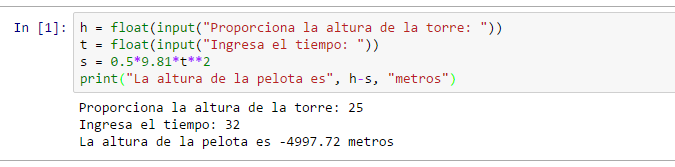
\includegraphics[scale=.8]{ca_da}
\end{figure}
\pagebreak

\section{Altitud}
En esta actividad se propone crear un programa que proporcione la altitud de un satèlite que orbita alrededor de la Tierra utilizando la ecuacion $(R+h)^3=(GMT^2)/(4\pi ^2)$. Se pide que el programa solicite el valor del periodo y arroje la altitud del satèlite en metros.
\subsection{Còdigo}

\begin{verbatim}
from math import pi
M=5.97e24
G=6.67e-11
R=6371e3
T=float(input("Ingrese el valor del periodo del satélite en minutos:"))
h=((G*M*((T*60)**2)*4*pi**2)**(1/3))+R
print("La altitud del satélite es de ",h,"metros")
\end{verbatim}
\subsection{Resultados}
\begin{figure}[H]
\centering
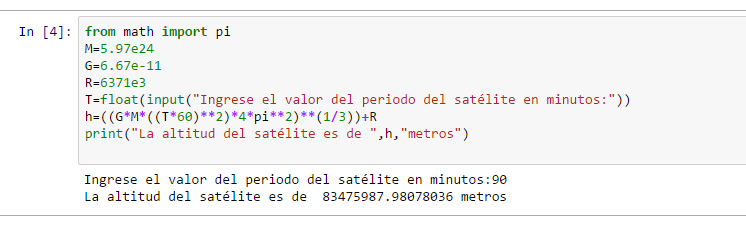
\includegraphics[scale=.8]{altitud}
\end{figure}
\pagebreak
\section{Polar}
En esta actividad se solicita crear un programa que arroje las coordenadas polares $(R,\theta,\phi)$ al ingresar las coordenadas cartesianas $(x,y,z)$.
\subsection{Còdigo}

\begin{verbatim}
from math import pi,atan,acos
x=float(input("Introduce x:"))
y=float(input("introduce y:"))
z=float(input("introduce z:"))
r= (x**2+y**2+z**2)**(1/2)
theta= atan(y/x)
phi= acos(z/r)
a=theta*180/pi
b=phi*180/pi
print("r=",r ,"theta=",a ,"phi=",b, )
\end{verbatim}

\subsection{Resultados}

	\begin{figure}[H]
	\centering
	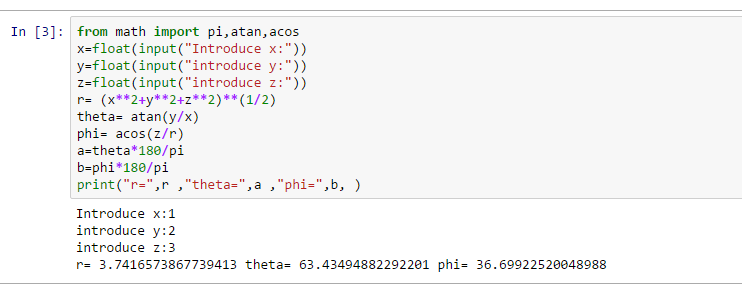
\includegraphics[scale=.8]{polar}
	\end{figure}
\pagebreak

\section{Even or odd}
En esta actividades proporcionado un còdigo por el profesor cuyo programa nos dice si el nùmero entero ingresado es par o impar. En èsta actividad se pretende comprender el uso del control"while".
\subsection{Còdigo}

\begin{verbatim}
print("Enter two integers, one even, one odd.")
m = int(input("Enter the first integer: "))
n = int(input("Enter the second integer: "))
while (m+n)%2==0:
    print("One must be even and the other odd.")
    m = int(input("Enter the first integer: "))
    n = int(input("Enter the second integer: "))
print("The numbers you chose are",m,"and",n)

\end{verbatim}

\subsection{Resultados}

\begin{figure}[H]
\centering
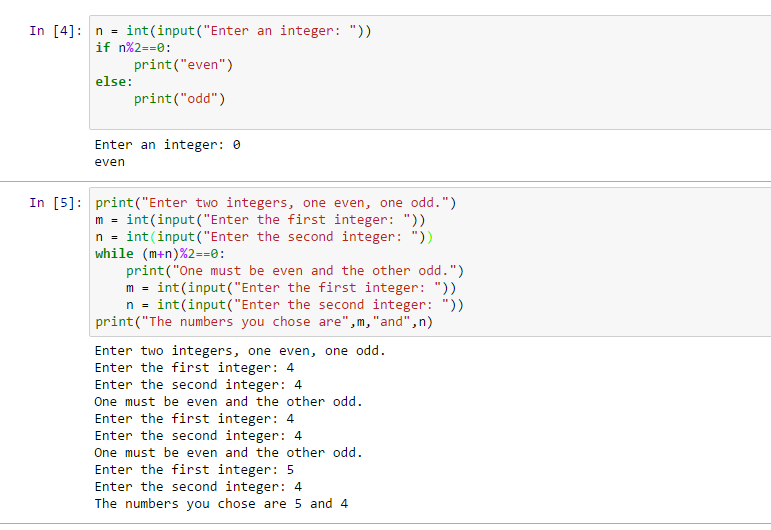
\includegraphics[scale=.8]{evenodd}
\end{figure}

\pagebreak

\section{Fibonacci}
En èsta actividad el profesor nos proporciona un còdigo para un programa que nos arroja la sucesiòn de nùmero fibonacci. êste còdigo funge como guìa para realizar otro similar el cual nos de como resultado la sucesiòn de nùmero de catalàn.

\subsection{Còdigo}

\begin{verbatim}

\end{verbatim}
\begin{verbatim}
n,C1,C2 = 0,1,1
while(C2 < 1000000): 
    print(C2)
    C2= C1*(4*n+2)/(n+2)
    n=n+1
    C1=C2
\end{verbatim}
\subsection{Resultados}

\begin{figure}[H]
\centering
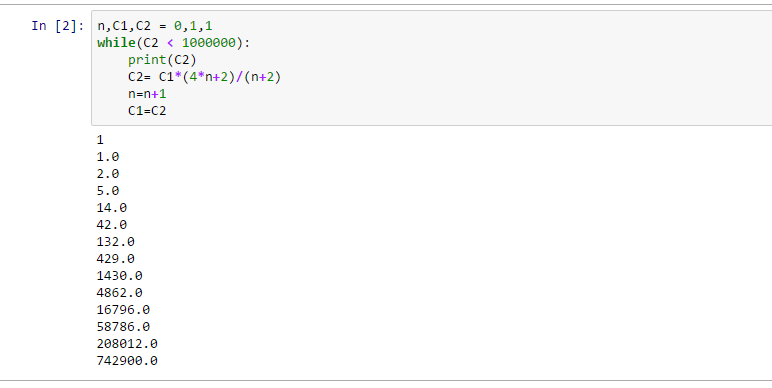
\includegraphics[scale=.8]{Fibonacci}
\end{figure}







\end{document}
